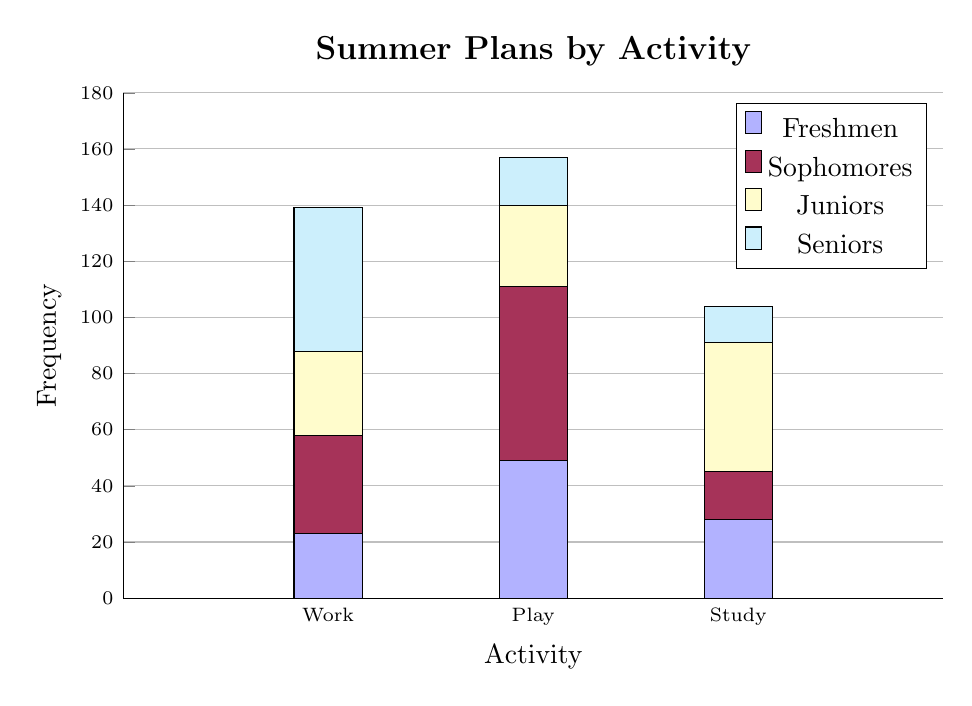
\begin{tikzpicture}[
    declare function={binom(\k,\n,\p)=\n!/(\k!*(\n-\k)!)*\p^\k*(1-\p)^(\n-\k);}
  ]
  \begin{axis}[
      axis lines*=left,
      no markers,
      xmin = 0, xmax=12, ymin=0, ymax=180,
      xtick={3,6,9},
      ytick={0,20,...,180}, 
      xticklabels={Work,Play,Study},
      ticklabel style={font=\scriptsize},
      xlabel={Activity},
      ylabel={Frequency},
      title={\large\bf Summer Plans by Activity},
      enlargelimits=false,
      clip=false,
      grid = none,
      ymajorgrids=true,
      ybar stacked,
      bar width=1,
      width=12cm,
      height=8cm
    ]
    \addplot+[draw=black,fill=blue!30] coordinates { 
        (3,23) (6,49) (9,28)
    };
    \addplot+[draw=black,fill=purple!60!gray] coordinates { 
        (3,35) (6,62) (9,17) 
    };
    \addplot+[draw=black,fill=yellow!20!white] coordinates { 
        (3,30) (6,29) (9,46)
    };
    \addplot+[draw=black,fill=cyan!20!white] coordinates { 
        (3,51) (6,17) (9,13)
    };
    \legend{\strut Freshmen, \strut Sophomores, \strut Juniors, \strut Seniors}
  \end{axis}
\end{tikzpicture}
